\section{METODOLOGIA}
%A metodologia proposta para alcançar os objetivos delineados é dividida em vários passos, que são descritos a seguir:

%Coleta e preparação dos dados: Realizar a coleta de um conjunto de imagens médicas contendo feridas malignas, garantindo a adequação ética e a privacidade dos pacientes. Preparar os dados, realizando a padronização, redimensionamento e possíveis ajustes de contraste ou iluminação, a fim de obter um conjunto de imagens consistente e pronto para o processamento.
%Pré-processamento das imagens: Aplicar técnicas de pré-processamento nas imagens médicas, como remoção de ruídos, normalização, equalização de histograma e segmentação preliminar, com o objetivo de melhorar a qualidade dos dados e fornecer informações mais relevantes para os modelos de aprendizado profundo.
%Implementação dos modelos de aprendizado profundo: Implementar os modelos de U-Net, SegNet, FCN e MobilenetV2 utilizando as bibliotecas e frameworks adequados para cada plataforma de machine learning: SageMaker, Azure Machine Learning e MLflow. Configurar os parâmetros necessários para cada modelo e realizar o treinamento utilizando o conjunto de dados preparados na etapa anterior.
%Avaliação do desempenho: Avaliar o desempenho de cada modelo treinado utilizando métricas estabelecidas, como acurácia, precisão, recall, F1-score e coeficiente de Dice. Realizar a comparação dos resultados obtidos por cada modelo em cada plataforma de machine learning, identificando os pontos fortes e fracos de cada arquitetura de aprendizado profundo.
%Avaliação da eficiência computacional: Analisar a eficiência computacional de cada modelo treinado nas diferentes plataformas, considerando métricas como tempo de treinamento, uso de recursos computacionais e escalabilidade. Compreender a capacidade de cada plataforma em lidar com o treinamento e inferência dos modelos em larga escala.
%Análise comparativa das arquiteturas: Realizar uma análise comparativa das diferentes arquiteturas de aprendizado profundo, considerando os resultados de desempenho e eficiência obtidos em cada plataforma. Identificar os modelos que apresentam melhores resultados e maior adequação para a tarefa de segmentação de feridas malignas em imagens médicas.
%Discussão e conclusões: Discutir os resultados obtidos, destacando as vantagens e limitações de cada modelo e plataforma de machine learning. Fornecer insights valiosos para futuras pesquisas na área de segmentação de imagens médicas utilizando aprendizado profundo. Concluir o estudo com uma síntese dos principais achados e destacar a relevância do projeto para a medicina, especialmente para a oncologia cutânea.
%Considerações éticas: Considerar as implicações éticas relacionadas à utilização de dados médicos sensíveis, garantindo a privacidade e confidencialidade dos pacientes envolvidos no estudo.
%Divulgação dos resultados: Documentar e apresentar os resultados do estudo em forma de relatório técnico-científico, artigos acadêmicos e/ou participação em conferências e workshops da área médica e de aprendizado de máquina.
%Aplicações futuras: Identificar possíveis aplicações práticas dos modelos


Este projeto de pesquisa emprega diversos modelos de aprendizagem profunda, tais como \ac{FCN}, \ac{U-Net}, \ac{SegNet} e \ac{MobileNetV2}, para segmentar feridas malignas em imagens médicas. Utilizaremos um grande conjunto de dados que reuniu uma junção de vários dataset de feridas. As imagens, que apresentam diversas formas e variações, serão pré-processadas antes do treinamento. Avaliaremos quantitativamente a performance dos modelos com base na área da ferida, precisão e eficiência do modelo na segmentação das imagens. A Figura~\ref{fig:diagrama} demonstra o fluxograma da metodologia aplicada.

\begin{figure}[H]
    \centering
    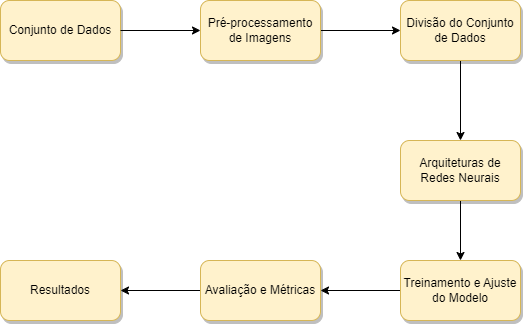
\includegraphics[width=0.8\textwidth]{img/Diagrama.png}
    \caption{Diagrama da Metodologia}
    \label{fig:diagrama}
\end{figure}

\subsection{Conjunto de Dados}
    O conjunto de dados deste estudo compreende imagens de feridas malignas coletadas de diversas fontes, incluindo repositórios públicos no GitHub e sites especializados em imagens médicas. Selecionamos mais de 4.800 imagens para treinar, validar e testar os modelos de aprendizado profundo, considerando a diversidade de tipos de feridas malignas e a qualidade das imagens. A utilização de um conjunto de dados amplo e diversificado contribuirá para aprimorar os resultados deste estudo e desenvolver modelos de aprendizado profundo mais eficazes na segmentação de feridas malignas.
    
\subsection{Criação do Conjunto de Dados}
    
    \begin{itemize}
        \item Tipo de imagens: As imagens médicas incluídas neste conjunto abrangem diversos tipos, tais Feridas de úlceras em pé diabéticos, lesões com cortes profundas e feridas cronicas em diversas partes do corpo. Suas características, como resolução, dimensões e formato de arquivo, são especificadas para proporcionar uma compreensão detalhada. Detalhamos o processo de aquisição, incluindo informações sobre o equipamento utilizado, configurações e protocolos adotados para a captura dessas imagens médicas.
    
        \item Pré-processamento e Anotação: Descrevemos as técnicas de pré-processamento aplicadas, como normalização e aumento de dados, ressaltando a importância dessas etapas na preparação das imagens para análise. O processo de anotação é abordado, incluindo responsáveis e critérios utilizados. Foi abordado nos dados sobre a diversidade do conjunto, considerando variabilidade em condições médicas, faixas etárias, gêneros e outros fatores relevantes, garantindo representatividade.
    
        \item Volume de Dados: Informamos a quantidade total de imagens e casos incluídos no dataset, proporcionando uma visão abrangente de sua robustez e amplitude. Consideramos mais de 4.800 imagens no dataset de diferentes fontes públicas e de diferentes condições clínicas para atender a heterogeneidade dos dados.
    
        \item Questões Éticas e de Privacidade: Abordamos as questões éticas, incluindo o consentimento informado, os processos de anonimização de dados e a conformidade com regulamentos de privacidade e proteção de dados.

        \item Qualidade e Confiabilidade dos Dados: Sobre a qualidade das imagens, considerando resolução e clareza, e a confiabilidade das anotações. Destacamos qualquer validação realizada por especialistas médicos para assegurar a precisão.

        \item Disponibilidade e Acesso: Fornecemos informações sobre a disponibilidade pública do dataset, incluindo detalhes sobre como acessá-lo, bem como eventuais restrições ou requisitos associados.

        \item Potenciais Aplicações e Limitações: Descrevemos possíveis aplicações do conjunto de dados em modelos de visão computacional, destacando suas potencialidades. Além disso, discutimos abertamente quaisquer limitações conhecidas ou possíveis viéses que devem ser considerados durante o uso do dataset.

        
    \end{itemize}

\subsection{Pré-processamento de Imagens}
    Primeiramente, as imagens foram redimensionadas para uma resolução de 256x256 pixels, a fim de padronizar o tamanho das imagens e facilitar o processamento pelos modelos. Em seguida, os valores de pixel foram normalizados para o intervalo [0, 1], a fim de garantir que todas as imagens tivessem a mesma escala de intensidade. 
    
    Além disso, foram aplicadas técnicas de aumento de dados, como rotação, inversão horizontal e zoom, para aumentar a diversidade do conjunto de dados e evitar overfitting. Essas técnicas permitem que os modelos aprendam a reconhecer as características das feridas malignas em diferentes posições e escalas.
    
    É importante destacar que não foram aplicados filtros de suavização nas imagens, a fim de preservar as características originais das feridas. Isso é importante para garantir que os modelos aprendam a reconhecer as características específicas das feridas malignas e não sejam influenciados por artefatos de imagem.
    
    Essas são etapa fundamental no treinamento de modelos de aprendizado profundo para a segmentação de feridas malignas. Ele permite que os modelos aprendam a reconhecer as características das feridas malignas de forma mais eficiente e precisa, resultando em segmentações mais precisas e confiáveis.

\subsection{Divisão do Conjunto de Dados}
    % Dividiremos o conjunto de dados de forma estratificada, assegurando uma distribuição uniforme das classes de feridas malignas em cada subconjunto. Destinaremos 80\% dos dados para treinamento, 10\% para validação e os 10\% restantes para testes. Essa divisão estratificada é crucial para garantir uma representação equilibrada das classes de feridas malignas e evitar viés nos resultados.

    A divisão do conjunto de dados foi realizada de forma estratificada, garantindo uma distribuição uniforme das classes de feridas malignas em cada subconjunto. Isso é importante para garantir que os modelos sejam treinados e avaliados em um conjunto de dados representativo e equilibrado, evitando viéses e garantindo resultados mais confiáveis.

    O conjunto de dados foi dividido em dois subconjuntos: treinamento e teste. O subconjunto de treinamento foi utilizado para treinar os modelos de aprendizado profundo, enquanto o subconjunto de teste foi utilizado para avaliar o desempenho dos modelos em dados não vistos anteriormente.

    A divisão do conjunto de dados foi realizada de forma aleatória, mas mantendo a proporção de cada classe de feridas malignas em cada subconjunto. Isso garante que os modelos sejam treinados e avaliados em um conjunto de dados representativo e equilibrado, evitando viéses e garantindo resultados mais confiáveis.

    Esses processos garantem que os modelos sejam treinados e avaliados em um conjunto de dados representativo e equilibrado, garantindo resultados mais confiáveis e precisos.

\subsection{Arquiteturas de Redes Neurais}
    Para realizar a segmentação das feridas malignas cutâneas, foram exploradas quatro arquiteturas de redes neurais convolucionais:

    \subsubsection{FCN}

        A arquitetura \ac{FCN} é conhecida por sua capacidade de realizar a segmentação semântica em imagens. Ela consiste em uma rede neural convolucional totalmente composta por camadas convolucionais, sem camadas totalmente conectadas. Essa arquitetura foi adaptada para realizar a segmentação precisa das feridas malignas cutâneas.

        \begin{figure}[H]
            \centering
            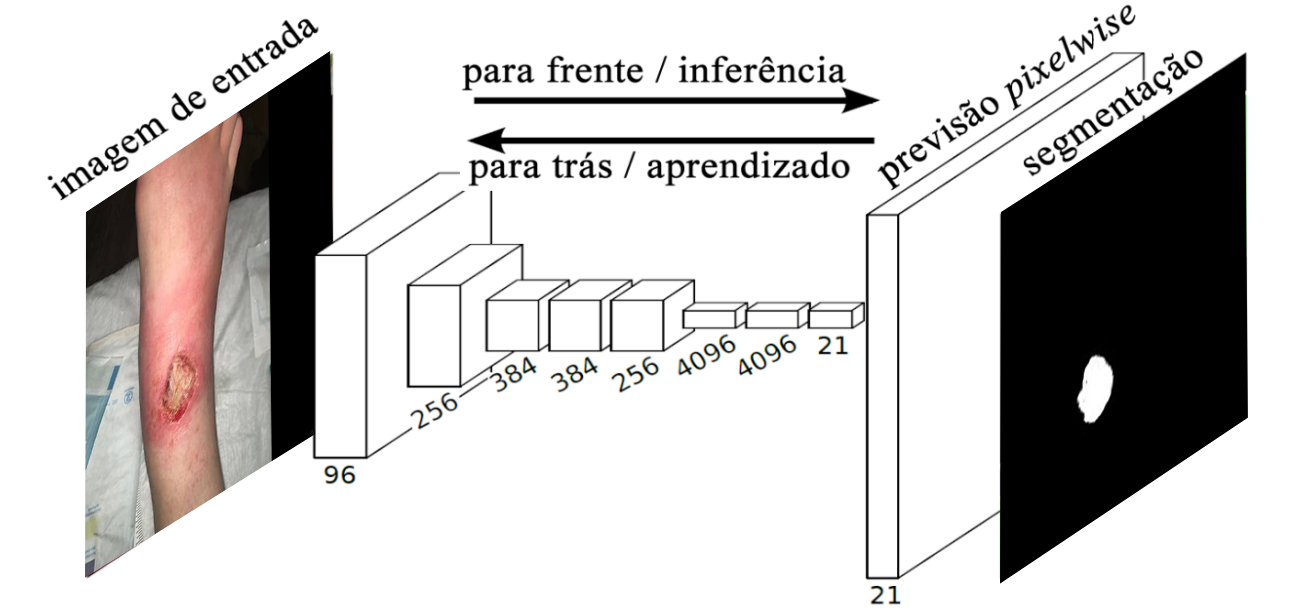
\includegraphics[width=0.9\textwidth]{img/arquitetura_FCN.png}
            \caption{Representação Esquemática da Arquitetura \ac{FCN}. adaptada de (\cite{long2015fully})}
            \label{fig:arquiteturaFCN}
        \end{figure}

        \begin{enumerate}
            \item A Figura \ref{fig:arquiteturaFCN} apresenta a arquitetura de uma rede \ac{FCN} utilizada para tarefa de segmentação semântica (semantic segmentation), isto é, classificar cada pixel da imagem de entrada de acordo com a classe que ele pertence, sendo: cama, pé ou ferida (background). Conforme a arquitetura apresentada na Figura, existem várias camadas de convolução que produzirão mapas de características de diferentes profundidades. No final da rede, encontra-se a previsão pixelwise (pixelwise prediction) que também é um tipo de camada de convolução e que irá fazer uma predição pixel-a-pixel, isto é, atribuindo cada pixel a uma respectiva classe. Esta representação ilustra de forma esquemática a arquitetura \ac{FCN}, mostrando as camadas convolucionais e suas dimensões. Essa arquitetura é capaz de extrair as características mais importantes das imagens de feridas malignas, permitindo que a rede aprenda a segmentar essas feridas com precisão. 
        \end{enumerate}

    
    \subsubsection{U-Net}

        A arquitetura \ac{U-Net} é amplamente utilizada para tarefas de segmentação em imagens biomédicas. Ela possui uma estrutura em forma de U, com um encoder para capturar informações contextuais e um decoder para reconstruir a máscara de segmentação. A \ac{U-Net} é conhecida por sua capacidade de segmentação precisa e é aplicada com sucesso em diversos problemas de segmentação, incluindo a segmentação de feridas medicas.

        \begin{figure}[H]
            \centering
            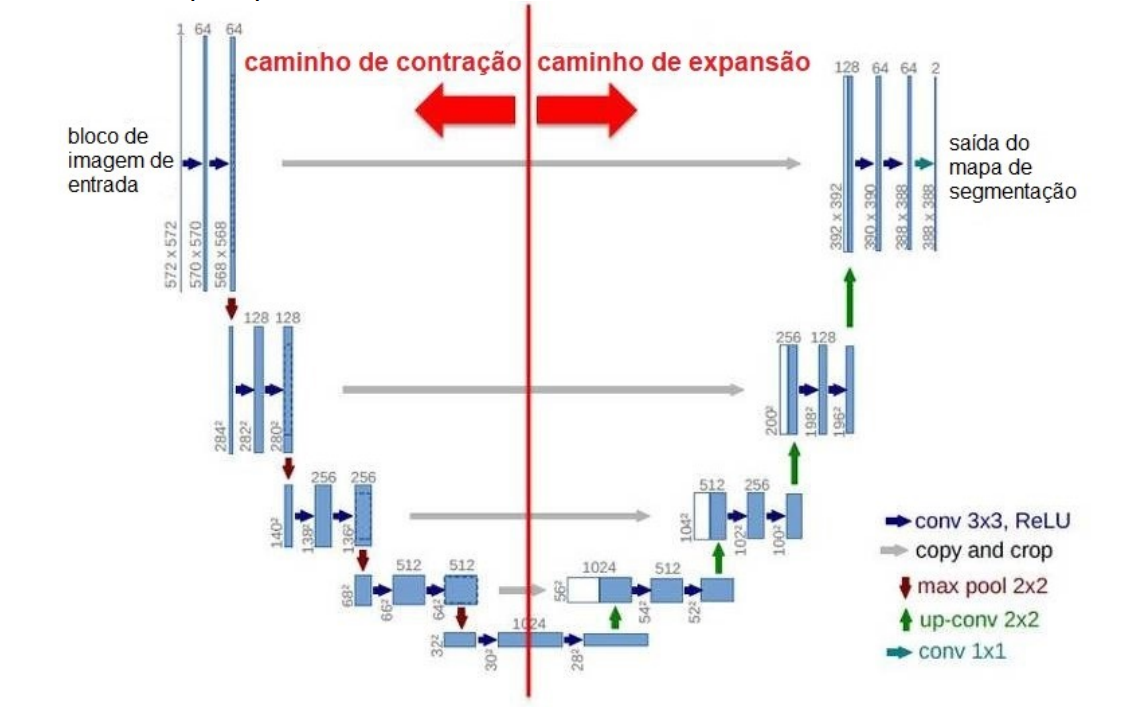
\includegraphics[width=0.9\textwidth]{img/arquitetura_U-Net.png}
            \caption{Representação Esquemática da Arquitetura \ac{U-Net}. adaptada de (\cite{ronneberger2015u})}
            \label{fig:arquiteturaUNet}
        \end{figure}

        \begin{enumerate}
            \item A Figura \ref{fig:arquiteturaUNet} ilustra a arquitetura da rede \ac{U-Net}, em que cada caixinha azul presente na imagem corresponde a um mapa de característica multicanal (multichannel feature map). O número de cada canal está descrito no valor acima de cada caixa. No canto inferior esquerdo é dada a dimensão x-y da imagem. As caixas brancas representam a cópia dos mapas de características (feature maps) e cada flecha com sua respectiva cor representa uma operação diferente. Na parte direita da rede as flechas verdes referem-se ao caminho de expansão onde é utilizado a operação de up-convolution, também chamada de de-convolution6 ou transposed convolution. A figura ilustra essa arquitetura de forma esquemática, mostrando as camadas convolucionais, as camadas de pooling máximo e up-sampling, e as conexões laterais entre as camadas do caminho de contração e do caminho de expansão.

        \end{enumerate}

    
    \subsubsection{SegNet}

        O modelo \ac{SegNet} é baseado em uma arquitetura de codificador-decodificador. Cada codificador aplica convolução, normalização de lote e uma não linearidade, e depois aplica um pool máximo no resultado, enquanto armazena o índice do valor extraído de cada janela. Os decodificadores são semelhantes aos codificadores, a diferença é que eles não têm uma não linearidade e aumentam a amostra de entrada, usando índices armazenados a partir do estágio de codificação. 

        \begin{figure}[H]
            \centering
            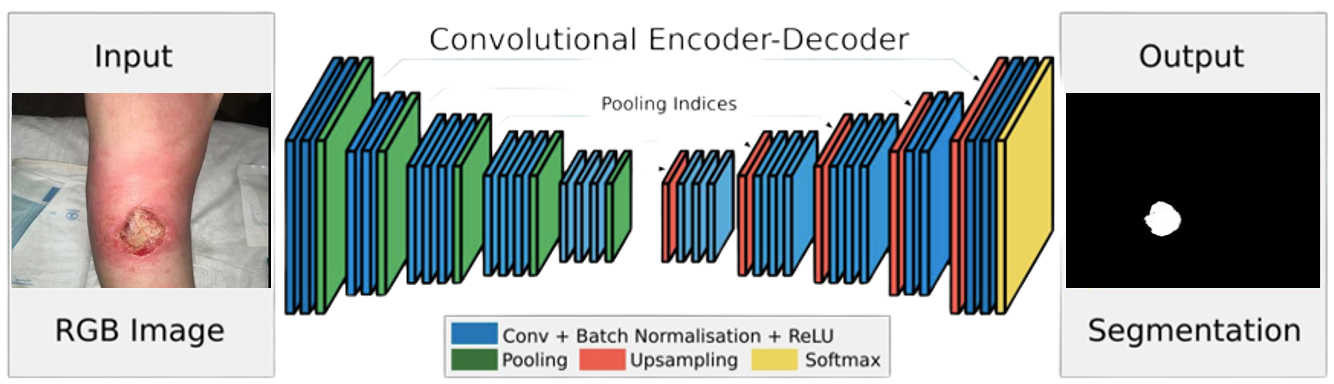
\includegraphics[width=0.9\textwidth]{img/arquitetura_Seg-Net.png}
            \caption{Representação Esquemática da Arquitetura \ac{SegNet}. adaptada de (\cite{badrinarayanan2017deep})}
            \label{fig:arquiteturaSegNet}
        \end{figure}

        \begin{enumerate}
            \item A Figura \ref{fig:arquiteturaSegNet} ilustra essa arquitetura de forma esquemática, mostrando as camadas de codificação e decodificação, bem como as conexões entre elas. Cada caixa na figura representa uma camada de convolução, normalização de lote e não linearidade, enquanto as setas representam as conexões entre as camadas. As camadas de pooling máximo são representadas pelas caixas de cor verde. Além disso, a figura também mostra a saída da rede, que é uma imagem segmentada com as áreas de feridas malignas destacadas em branco. Essa saída é gerada pela última camada de decodificação da rede.
            Em resumo, a Figura ilustra de forma esquemática a arquitetura \ac{SegNet}, mostrando as camadas de codificação e decodificação, bem como as conexões entre elas. Essa arquitetura é capaz de segmentar com precisão as feridas malignas em imagens médicas, como mostrado nos resultados do estudo.
        \end{enumerate}

    
    \subsubsection{MobileNetV2}

        O \ac{MobileNetV2} é uma arquitetura de rede neural convolucional projetada para tarefas de classificação e segmentação em dispositivos com recursos computacionais limitados. Essa arquitetura utiliza camadas convolucionais separáveis em profundidade para obter um bom equilíbrio entre a precisão do modelo e a eficiência computacional.
    
            \begin{figure}[H]
                \centering
                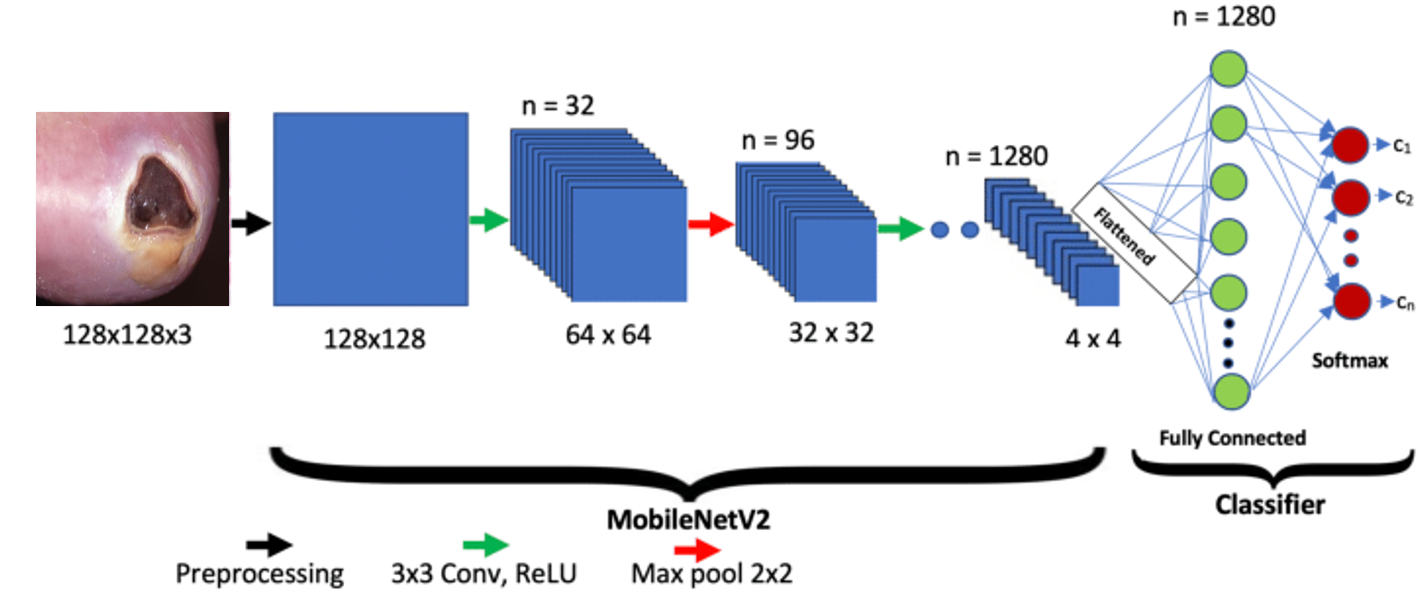
\includegraphics[width=0.9\textwidth]{img/arquitetura_MobileNetV2.png}
                \caption{Representação Esquemática da Arquitetura \ac{MobileNetV2}. adaptada de (\cite{akay2021deep})}
                \label{fig:arquiteturaMobileNetV2}
            \end{figure}
            
    
            \begin{enumerate}
                \item A Figura \ref{fig:arquiteturaMobileNetV2} ilustra essa arquitetura de forma esquemática, mostrando as camadas convolucionais e suas dimensões. A imagem de entrada é uma imagem de ferida com dimensões 128x128x3, que é processada pela primeira camada convolucional com dimensões 128x128 e um número de filtros (ou canais) igual a 32. Em seguida, a imagem é processada por uma segunda camada convolucional com dimensões 64x64 e um número de filtros igual a 32. Depois disso, a imagem é processada por várias camadas convolucionais com dimensões 32x32 e 96 filtros, que são responsáveis por extrair características mais complexas da imagem. Essas camadas são seguidas por uma camada convolucional com dimensões 4x4 e um número de filtros igual a 1280, que é responsável por extrair as características mais importantes da imagem. Por fim, a saída da última camada convolucional é processada por uma rede fully connected com um número de neurônios igual a 1280, que é responsável por gerar a saída final da rede.
                Em resumo, a Figura ilustra de forma esquemática a arquitetura \ac{MobileNetV2}, mostrando as camadas convolucionais e suas dimensões. Essa arquitetura é capaz de extrair as características mais importantes das imagens de feridas malignas, permitindo que a rede aprenda a segmentar essas feridas com precisão. 
            \end{enumerate}

\subsection{Treinamento e Ajuste do Modelo}
    Durante o processo de treinamento, utilizamos um conjunto de imagens de feridas malignas criado para ensinar os modelos a segmentar essas feridas com precisão. Para isso, dividimos o conjunto de imagens em conjuntos de treinamento e teste, e utilizamos técnicas de data augmentation para aumentar a diversidade do conjunto de treinamento.

    Além disso, aplicamos técnicas de poda nos modelos abordados, com o objetivo de reduzir o número de parâmetros e melhorar a eficiência computacional dos modelos. A técnica de poda consiste em remover os pesos menos importantes dos modelos, mantendo apenas os pesos mais importantes. Isso permite que os modelos sejam mais eficientes em termos de memória e processamento, sem comprometer a precisão da segmentação.

    Durante o processo de ajuste, utilizamos o conjunto de dados para ajustar os hiperparâmetros dos modelos e evitar overfitting. Ajustamos os hiperparâmetros como taxa de aprendizado, tamanho do batch e número de épocas de treinamento, com o objetivo de obter a melhor precisão de segmentação possível.

\subsection{Avaliação e Métricas}
    Na avaliação do desempenho dos modelos de segmentação de feridas malignas em imagens médicas, foram aplicadas diversas métricas fundamentais. A métrica de Loss, foi utilizada para quantificar a diferença entre a segmentação prevista pelo modelo e as segmentações reais. Esse indicador é crucial para o ajuste e a otimização dos modelos, sendo que valores menores de Loss indicam uma segmentação mais precisa.

    Além disso, a métrica Dice, frequentemente empregada em tarefas de segmentação, avalia a sobreposição entre a segmentação prevista e a verdade de referência. Valores mais próximos de 1 indicam uma sobreposição ideal entre as segmentações.

    Precision e Recall são métricas fundamentais para avaliar a precisão do modelo em identificar corretamente as feridas malignas. A Precision foi usada para mensura a proporção de verdadeiros positivos em relação ao total de predições positivas, enquanto o Recall mediu a capacidade do modelo em identificar corretamente todas as instâncias de feridas malignas, minimizando falsos negativos.

    A combinação dessas métricas proporciona uma visão abrangente do desempenho dos modelos, permitindo ajustes precisos e identificação de áreas para melhoria. Valores ideais dessas métricas variam de acordo com as necessidades clínicas e são cruciais para garantir a confiabilidade dos resultados obtidos na segmentação.

    Além dessas métricas, também calculamos a área da ferida para fornecer uma medida quantitativa da extensão das feridas segmentadas. Realizamos testes t para verificar as diferenças significativas entre as métricas dos modelos e realizamos análises estatísticas dos resultados usando testes estatísticos adequados.

    Essas métricas foram escolhidas porque fornecem uma avaliação abrangente do desempenho dos modelos em diferentes aspectos, como acurácia, completude e similaridade com a segmentação manual. Além disso, a área da ferida foi calculada para fornecer uma medida quantitativa da extensão das feridas segmentadas. A análise estatística dos resultados foi realizada para verificar se as diferenças observadas entre os modelos eram estatisticamente significativas. Em resumo, as métricas utilizadas neste contexto do trabalho foram escolhidas para fornecer uma avaliação abrangente e precisa do desempenho dos modelos de segmentação de feridas malignas em imagens médicas.

\subsection{Considerações Éticas}
    Dada a natureza das imagens médicas de pacientes, atenderemos rigorosamente às considerações éticas. Anonimizaremos todas as imagens, removendo informações identificáveis para assegurar a privacidade dos pacientes. Este projeto caminhou para atender as diretrizes da Declaração de Helsinque para pesquisas envolvendo seres humanos. Essa declaração é um conjunto de princípios éticos que orientam a pesquisa médica envolvendo seres humanos. Ela foi criada para proteger os direitos, a segurança e o bem-estar dos pacientes envolvidos em pesquisas médicas.
    
    A implementação desta metodologia permitirá avaliar a eficácia de vários modelos de aprendizagem profunda na segmentação de feridas malignas em imagens médicas. Compararemos os modelos usando uma variedade de métricas para fornecer insights valiosos para o desenvolvimento de futuros sistemas de diagnóstico assistido por computador na área de oncologia cutânea.

